\documentclass[article,12pt]{elsarticle}
\usepackage[utf8]{inputenc}
\usepackage{graphicx}
\usepackage{booktabs}
\usepackage{subcaption}
\usepackage{amssymb}
\usepackage{flushend}
\usepackage{float}
\usepackage{amsmath}
\usepackage{amsfonts}
\usepackage{dcolumn}
\usepackage{amsthm}
\usepackage{caption}
\usepackage{lmodern}
\usepackage{booktabs}
\usepackage{color}
\usepackage{longtable}
\usepackage{rotating}
\usepackage{etoolbox}
\usepackage{hyperref}
\usepackage{comment}
\usepackage{pdflscape}
\usepackage{comment}
\usepackage[table,xcdraw]{xcolor}
\usepackage[framemethod=TikZ]{mdframed}
\usepackage[a4paper, left=1.5cm, right=1.5cm, top=2cm, bottom=2cm]{geometry}

\begin{document}

\mdfsetup{innertopmargin=10pt,linecolor=blue!20,%
linewidth=2pt,topline=true,
frametitleaboveskip=\dimexpr-\ht\strutbox\relax,}

\begin{frontmatter}
    \title{Laboratorio de Óptica \\  Práctica  I: Radiometría}
    \author{López González Andrés$^1$, Reyes Saldivar Ailton Uriel$^2$ y Gante Morales Pedro José$^3$} %Aquí va el nombre de los integrantes que participaron en el informe.
    \address{$^1$ Facultad de Ciencias, Universidad Nacional Autónoma de México, M\'exico CDMX.}

\begin{abstract}
La radiometría es la rama de la óptica que estudia la propagación y distribución energética de la luz en función de magnitudes como flujo radiante, irradiancia, intensidad radiante y radiancia. En este experimento, se estudió la relación entre la irradiancia y la distancia a la fuente luminosa para dos tipos de emisores: un LED y un láser. Se realizaron mediciones variando la distancia entre el sensor de irradiancia y la fuente en incrementos de ($5 \pm 2$)mm, ($10 \pm 2$)mm y ($50 \pm 2$)mm. Se compararon los resultados con dos modelos teóricos: la ley del inverso del cuadrado, que predice que la irradiancia de una fuente perfectamente puntual disminuye con \( r^{-2} \), y el modelo de haz colimado, en el que la irradiancia es constante. Los resultados experimentales mostraron que el LED sigue la tendencia de la ley del inverso del cuadrado con un exponente de decaimiento \( m = -1.94 \pm 0.00647 \), mientras que el láser presenta un exponente significativamente menor, \( m = -0.0182 \pm 0.00167 \), indicando una propagación casi colimada (i.e., de divergencia tendiendo a cero para distancias de hasta 400mm acorde a este estudio). Estos resultados validan la dependencia de la irradiancia con la naturaleza de la fuente y confirman la aplicabilidad de los modelos radiométricos en la caracterización de fuentes de luz.
\end{abstract}
    
\end{frontmatter}

\vspace{0.5cm} 

\section{Introducción}
La radiometría es la rama de la óptica que estudia y cuantifica la propagación de la luz en términos de su energía e intensidad dentro del espectro electromagnético, que abarca longitudes de onda desde los 10 nm hasta los 1000 $\mu$m. Existen cuatro magnitudes fundamentales en radiometría que permiten describir el comportamiento de la luz:

\begin{itemize}
\item \textbf{Flujo de Radiación} $\Phi$ [W]: Es la tasa de flujo de energía por unidad de tiempo:

\begin{mdframed}
\begin{equation}
\Phi = \frac{dQ}{dt}
\end{equation}
\end{mdframed}

\item \textbf{Irradiancia} $I$ [W/m²]: Es la densidad de flujo de radiación por unidad de área en una superficie:

\begin{mdframed}
\begin{equation}
    I = \frac{d\Phi}{ds_0}
\end{equation}
\end{mdframed}

donde $ds_0$ es un elemento de área sobre la superficie de estudio.

\item \textbf{Intensidad Radiante} $E$ [W/sr]: Se define como el flujo por unidad de ángulo sólido:

\begin{mdframed}
\begin{equation}
    E = \frac{d\Phi}{d\omega}
\end{equation}
\end{mdframed}

donde $d\omega$ es un elemento de ángulo sólido.

\item \textbf{Radiancia} $L$ [W/m²sr]: Representa la densidad de flujo por unidad de área proyectada y por unidad de ángulo sólido:

\begin{mdframed}
\begin{equation}
    L = \frac{d^2\Phi}{ds_0 d\omega} = \frac{d^2\Phi}{ds \cos\theta d\omega}
\end{equation}
\end{mdframed}

donde $ds$ es la proyección del área $ds_0$ en la dirección del ángulo sólido $d\omega$.

\end{itemize}

El flujo total de radiación se obtiene integrando la radiancia sobre el área de detección y el ángulo sólido:

\begin{mdframed}
\begin{equation}
\Phi = \int_A \int_{\Omega} L(x,y,\theta,\phi) \cos\theta d\omega ds_0
\end{equation}
\end{mdframed}

Para describir la propagación de la luz desde una fuente, se consideran dos modelos teóricos principales: la propagación según la \textbf{ley del inverso del cuadrado} y la propagación mediante un \textbf{haz colimado}.

\subsection{Ley del Inverso del Cuadrado}

Cuando una fuente de luz puede aproximarse como puntual y la distancia entre la fuente y el detector es suficientemente grande (por convención, esto es cuando la diagonal de mayor tamaño de la fuente luminosa es a lo más $\frac{R}{20}$, en donde R es la distancia entre la fuente y el sensor), la irradiancia sigue la ley del inverso del cuadrado:

\begin{mdframed}
\begin{equation}
I_{Det} = \frac{K}{R^2}
\end{equation}
\end{mdframed}

donde $K$ es una constante y $R$ la distancia entre la fuente y el detector. Esta relación se deduce a partir de la geometría de emisión y la conservación del flujo radiante.

\subsection{Haz Colimado}

Para un haz colimado, la radiancia se mantiene constante en la dirección de propagación, lo que implica que la irradiancia no depende de la distancia:

\begin{mdframed}
\begin{equation}
I = L_0
\end{equation}
\end{mdframed}

donde $L_0$ es la radiancia constante del haz.

Dado que las fuentes reales no son perfectamente puntuales ni perfectamente colimadas, en la práctica la irradiancia sigue un modelo generalizado:

\begin{mdframed}
\begin{equation}
I = K r^m
\end{equation}
\end{mdframed}

donde $m$ es el \textbf{exponente de decaimiento} tal que $m \in [0,2]$, su valor es monótono creciente en cuanto su divergencia comienza a aumentar (de aquí se muestra que una fuente perfectamente colimada tendría divergencia cero y por ende exponente cero); en este estudio, consideraremos que un sistema sigue la "Ley del Inverso del Cuadrado" cuando su exponente \( m \) se aproxima a 2 desde valores ligeramente menores. Por otro lado, clasificaremos como "Haz Colimado" aquellos casos en los que el exponente de la distancia tienda a cero desde valores ligeramente positivos.

\begin{comment}
En este experimento se estudió la propagación de la luz de un LED y un láser, encontrando que:
\begin{itemize}
\item Para el LED: $I(r) \propto r^{-2.00 \pm 0.02}$, lo que concuerda con la ley del inverso del cuadrado.
\item Para el láser: $I(r) \propto r^{-0.081 \pm 0.006}$, lo que indica un haz casi colimado.
\end{itemize}

Estos resultados confirman que la propagación de la luz depende de la naturaleza de la fuente y permiten validar los modelos teóricos de radiometría.
\end{comment}

\subsection{Hipótesis}

La irradiancia de una fuente de luz depende de la distancia a la que se mide. En el caso de una \textbf{fuente puntual}, se espera que la irradiancia siga la \textbf{Ley del Inverso del Cuadrado}, es decir, que la relación entre la irradiancia \( I \) y la distancia \( r \) siga la forma:

\begin{mdframed}
\begin{equation}
    I(r) \propto r^{-2}
\end{equation}
\end{mdframed}

Por otro lado, para un \textbf{haz colimado} (como un láser), la irradiancia debería mantenerse aproximadamente constante con la distancia, siguiendo el modelo:

\begin{mdframed}
\begin{equation}
    I(r) \propto r^{0}
\end{equation}
\end{mdframed}

\subsection{Objetivos}

Se busca medir la irradiancia de una fuente puntual y un haz colimado a distintas distancias, determinar su relación funcional con la distancia mediante la ecuación \( I(r) = K r^m \), comparar el exponente \( m \) obtenido con los valores teóricos esperados y evaluar la validez del modelo considerando posibles errores experimentales.


\section{Desarrollo Experimental}
Para esté expereimento utilizamos dos tipos de fuentes: Un LED (fuente puntual) y un Láser(haz colimado) las cuales con ayuda de un porte y un porta poste se mantubieron fijas en la base de un riel. También utilizamos un radiometro para medir la irradiancia cuya mecición esta dada en [mW/m$^2$] o [W/m$^2$] que depende de la irrandiancia que este detectando ademas la incertidumbre asociada a este instrumento es otorgada por este mismo y puede variar dependiendo de la escala de la medición.

Para medir la distancia entre la fuente y el detector del radiometro utilizamos un riel con carro movil con graducacion en [mm] por tanto le asignamos una incertidumbre de apreciación de 0.5mm ademas notamos que la fuente de luz y el detector no se encontraban completamente centradas en el carro del riel por lo que decidimos agregar una incertidumbre de definicon de 2mm.

\subsection{Caso LED}
Con ayuda de un poste y un porta poste se dejo fijo al LED en el origen del riel mientras que el detector se coloco sobre un carro movil, además nos aseguramos de que el LED y el detector estuvieran a la misma altura. Para comenzar a medir nuestras irradiancias colocamos el detecor a una distancia de 40mm del LED porteriromente encendimos el LED para medir la irradiancia a esa distancia, una vez medida esa irradiancia pagamos el LED y medimos la irradiancia de fondo. Repetimos este procedimiento a diferentes distancias como se muestra en la Tabla 1.
Durante estas mediciones notamos que apartir de 250mm la medición de la irradiancia mostrada por el radiomentro fluctuaba mucho, por lo que decidimos tomar la medida promedio entre la mas grande y la mas pequeña. 

\subsection{Caso Láser}
Para este caso nuevamente utilizamos el mismo arreglo que en el caso anterior pero esta se tuvo que alinear el Láser de tal fotma que apunte en el centro del detector. A demás realizamos las mediciones a esas mismas distancias, solo que en este caso cada vez que recorriamos el detector, el Láser se desalineaba por lo que fue necesario alinearlo en cada una de las mediciones haciendo uso de los tornillos que tiene en la parte trasera del Láser sin embargo a pesar de esto era muy complicado alinearlo en su totalidad y por tanto decidimos registrar el valor máximo de la irradiancia que detectamos para cada una de las distancias.  

\begin{figure}[H]
    \centering
    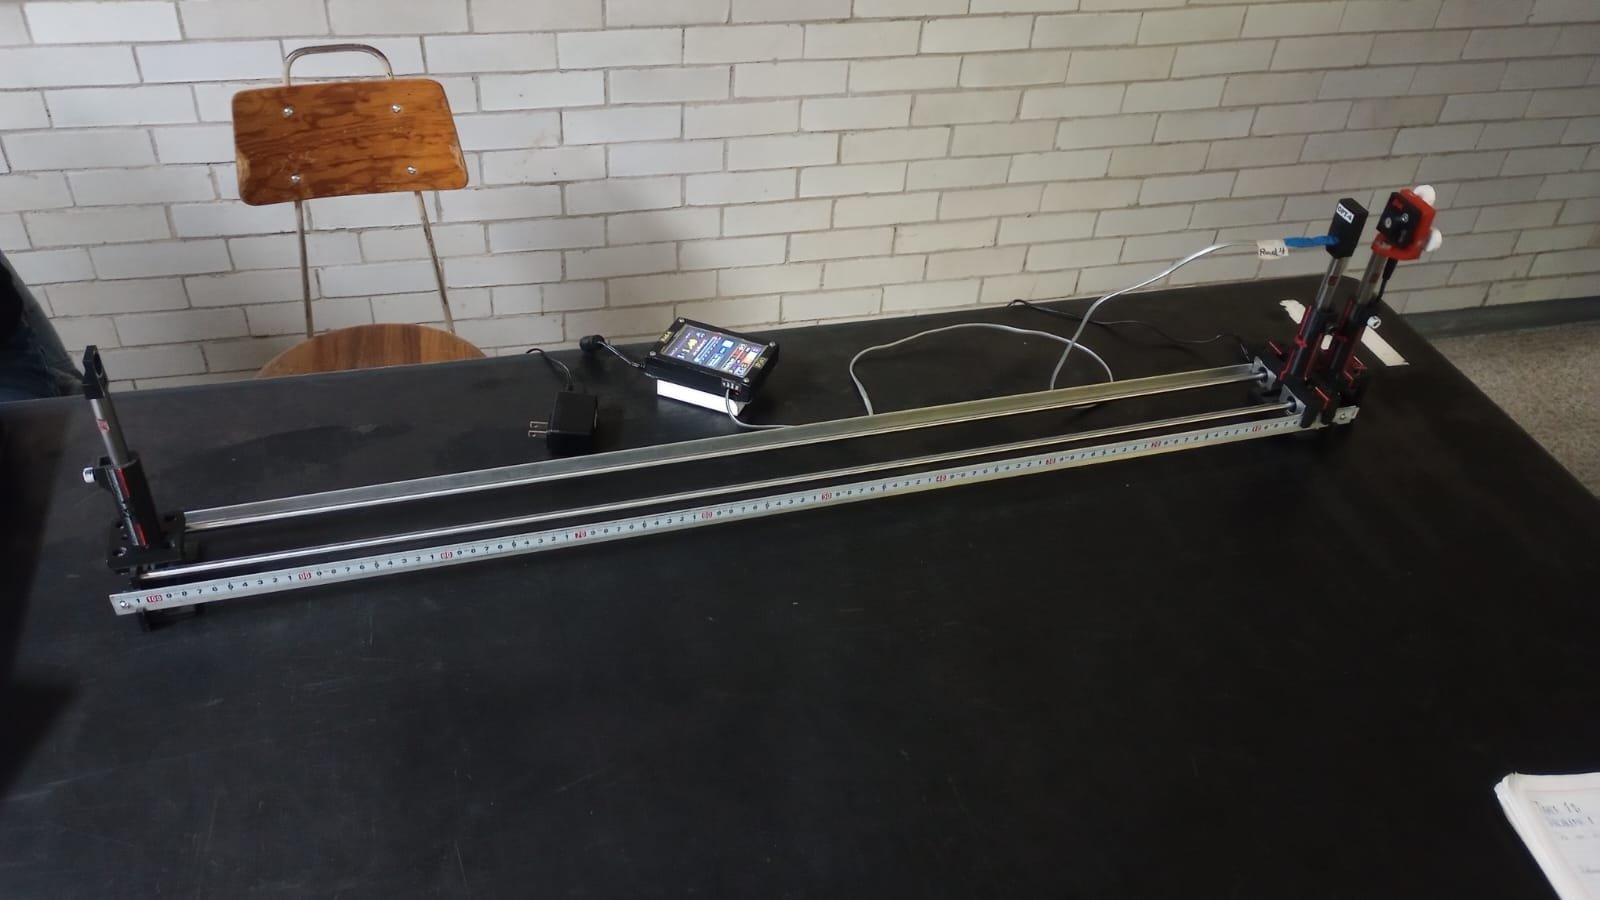
\includegraphics[width=0.5\linewidth]{DE P1 OPT.jpg}
    \caption{Arreglo experimental (caso láser)}
    \label{fig:enter-label}
\end{figure}


\input{Experimental Dev}

\section{Resultados y discusión}
\subsection{Fuente puntual}

A continuación se muestras los resultados de cómo varía la irradiancia con respecto a la distancia en el caso del LED (fuente puntual)\\

\begin{table}[h]
\centering
\begin{tabular}{
>{\columncolor[HTML]{C5E0B3}}c 
>{\columncolor[HTML]{FFE598}}c 
>{\columncolor[HTML]{C5E0B3}}c 
>{\columncolor[HTML]{FFE598}}c 
>{\columncolor[HTML]{BDD6EE}}c 
>{\columncolor[HTML]{FFE598}}c l
>{\columncolor[HTML]{C5E0B3}}c 
>{\columncolor[HTML]{FFE598}}c 
>{\columncolor[HTML]{C5E0B3}}c 
>{\columncolor[HTML]{FFE598}}c }
\multicolumn{6}{c}{\cellcolor[HTML]{FFEB9C}{\color[HTML]{9C6500} Fuente Puntual}}                                                                                                                                          &  & \multicolumn{4}{c}{\cellcolor[HTML]{FFEB9C}{\color[HTML]{9C6500} Linealización}}                                                        \\
\cellcolor[HTML]{92D050}r ($mm$) & \cellcolor[HTML]{FFC000}Δr ($mm$) & \cellcolor[HTML]{92D050}I ($\frac{mW}{m^2}$) & \cellcolor[HTML]{FFC000}ΔI ($\frac{mW}{m^2}$) & \cellcolor[HTML]{DEEAF6}Fondo ($\frac{mW}{m^2}$) & \cellcolor[HTML]{FFC000}I real ($\frac{mW}{m^2}$) &  & \cellcolor[HTML]{92D050}lin(r) & \cellcolor[HTML]{FFC000}Δ(lin(r)) & \cellcolor[HTML]{92D050}lin(I) & \cellcolor[HTML]{FFC000}Δ(lin(I)) \\
40                             & 2                               & 350                               & 10                                 & 0.5                                   & 349.50                                 &  & 3.69                           & 0.05                              & 5.86                           & 0.03                              \\
45                             & 2                               & 290                               & 10                                 & 0.5                                   & 289.50                                 &  & 3.81                           & 0.04                              & 5.67                           & 0.03                              \\
50                             & 2                               & 230                               & 10                                 & 0.46                                  & 229.54                                 &  & 3.91                           & 0.04                              & 5.44                           & 0.04                              \\
55                             & 2                               & 190                               & 10                                 & 0.48                                  & 189.52                                 &  & 4.01                           & 0.04                              & 5.25                           & 0.05                              \\
60                             & 2                               & 160.00                            & 10                                 & 0.46                                  & 159.54                                 &  & 4.09                           & 0.03                              & 5.08                           & 0.06                              \\
65                             & 2                               & 140.00                            & 10                                 & 0.44                                  & 139.56                                 &  & 4.17                           & 0.03                              & 4.94                           & 0.07                              \\
70                             & 2                               & 117.10                            & 1                                  & 0.44                                  & 116.66                                 &  & 4.25                           & 0.03                              & 4.76                           & 0.01                              \\
75                             & 2                               & 102.60                            & 1                                  & 0.46                                  & 102.14                                 &  & 4.32                           & 0.03                              & 4.63                           & 0.01                              \\
80                             & 2                               & 89.70                             & 1                                  & 0.48                                  & 89.22                                  &  & 4.38                           & 0.03                              & 4.50                           & 0.01                              \\
85                             & 2                               & 79.80                             & 1                                  & 0.46                                  & 79.34                                  &  & 4.44                           & 0.02                              & 4.38                           & 0.01                              \\
90                             & 2                               & 71.10                             & 1                                  & 0.48                                  & 70.62                                  &  & 4.50                           & 0.02                              & 4.26                           & 0.01                              \\
100                            & 2                               & 57.80                             & 1                                  & 0.46                                  & 57.34                                  &  & 4.61                           & 0.02                              & 4.06                           & 0.02                              \\
110                            & 2                               & 48.50                             & 1                                  & 0.46                                  & 48.04                                  &  & 4.70                           & 0.02                              & 3.88                           & 0.02                              \\
120                            & 2                               & 41.20                             & 1                                  & 0.46                                  & 40.74                                  &  & 4.79                           & 0.02                              & 3.72                           & 0.02                              \\
130                            & 2                               & 34.50                             & 1                                  & 0.44                                  & 34.06                                  &  & 4.87                           & 0.02                              & 3.54                           & 0.03                              \\
140                            & 2                               & 30.40                             & 1                                  & 0.44                                  & 29.96                                  &  & 4.94                           & 0.01                              & 3.41                           & 0.03                              \\
150                            & 2                               & 26.50                             & 1                                  & 0.44                                  & 26.06                                  &  & 5.01                           & 0.01                              & 3.28                           & 0.04                              \\
200                            & 2                               & 15.50                             & 1                                  & 0.44                                  & 15.06                                  &  & 5.30                           & 0.01                              & 2.74                           & 0.07                              \\
250                            & 2                               & 9.75                              & 0.5                                & 0.44                                  & 9.31                                   &  & 5.52                           & 0.01                              & 2.28                           & 0.05                              \\
300                            & 2                               & 6.91                              & 0.5                                & 0.46                                  & 6.45                                   &  & 5.70                           & 0.01                              & 1.93                           & 0.08                              \\
350                            & 2                               & 5.26                              & 0.5                                & 0.46                                  & 4.80                                   &  & 5.86                           & 0.01                              & 1.66                           & 0.10                              \\
400                            & 2                               & 4.17                              & 0.5                                & 0.5                                   & 3.67                                   &  & 5.99                           & 0.01                              & 1.43                           & 0.14                             
\end{tabular}
\caption{Tabla de Distancia vs Irradiancia y linealización para la fuente puntual con incertidumbres}
\label{tab:my-table}
\end{table}\\

Al realizar la aproximación potencial en $R$ vs $I$, y la regresión lineal a $\ln R$ vs $\ln I$ obtenemos los siguientes gráficos.\\

\begin{figure}[H]
    \centering
    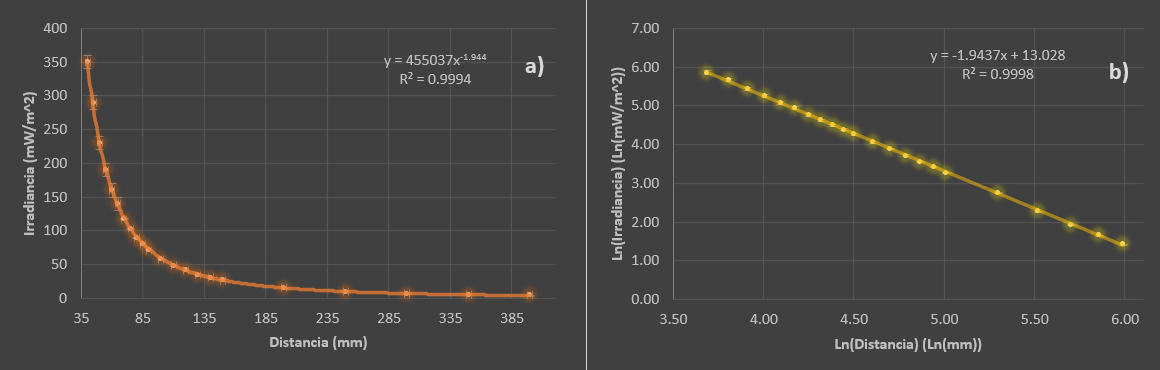
\includegraphics[width=1\linewidth]{Ajuste PL puntual.png}
    \caption{a) Gráfico d vs R con incertidumbres \qquad b) Gráfico ln(d) vs ln(R) con incertidumbres}
    \label{fig:enter-label}
\end{figure}\\

Nótese que obtenemos una expresión de la irradiancia de la forma $I = 455037r^{-1.944} \approx \lim_{m\rightarrow2^-} \dfrac{\Gamma_0}{r^2}$. Por lo que podemos asumir que el LED es una fuente puntual pues se ha cumplido la Ley del Inverso al Cuadrado; por otro lado en el gráfico linealizado obtuvimos la ecuación $\ln I = -1.944 \ln r + 13.028$, de aquí es más sencillo obtener la incertidumbre de m que acorde a los parámetros de la regresión lineal $\Delta m = 0.00646793 \approx 0.006
$. De modo que finalmente nuestra irradiancia del LED queda determinada por

\begin{mdframed}
    \begin{equation}
        I = \frac{455037}{r^{1.944\pm0.006}}
    \end{equation}
\end{mdframed}

\subsection{Haz colimado}

A continuación se muestras los resultados de cómo varía la irradiancia con respecto a la distancia en el caso del Laser (haz colimado)\\

\begin{table}[h]
\centering
\begin{tabular}{
>{\columncolor[HTML]{C5E0B3}}c 
>{\columncolor[HTML]{FFE598}}c 
>{\columncolor[HTML]{C5E0B3}}c 
>{\columncolor[HTML]{FFE598}}c 
>{\columncolor[HTML]{BDD6EE}}c 
>{\columncolor[HTML]{FFE598}}c c
>{\columncolor[HTML]{C5E0B3}}c 
>{\columncolor[HTML]{C5E0B3}}c 
>{\columncolor[HTML]{C5E0B3}}c 
>{\columncolor[HTML]{C5E0B3}}c }
\multicolumn{6}{c}{\cellcolor[HTML]{FFEB9C}{\color[HTML]{9C6500} Fuente   Laser}}                                                                                                                                                  & {\color[HTML]{9C6500} } & \multicolumn{4}{c}{\cellcolor[HTML]{FFEB9C}{\color[HTML]{9C6500} Linealización}}                                                        \\
\cellcolor[HTML]{92D050}r ($mm$) & \cellcolor[HTML]{FFC000}Δr ($mm$) & \cellcolor[HTML]{92D050}I ($\frac{mW}{m^2}$) & \cellcolor[HTML]{FFC000}ΔI ($\frac{mW}{m^2}$) & \cellcolor[HTML]{DEEAF6}Fondo ($\frac{mW}{m^2}$) & \cellcolor[HTML]{FFC000}I real ($\frac{mW}{m^2}$) &  & \cellcolor[HTML]{92D050}lin(r) & \cellcolor[HTML]{FFC000}Δ(lin(r)) & \cellcolor[HTML]{92D050}lin(I) & \cellcolor[HTML]{FFC000}Δ(lin(I)) \\
40                             & 2                               & 6830                                & 50                                   & 0.46                                    & 6830                                     &                         & 3.69                           & 0.05                              & 8.83                           & 0.01                              \\
45                             & 2                               & 6850                                & 50                                   & 0.48                                    & 6850                                     &                         & 3.81                           & 0.04                              & 8.83                           & 0.01                              \\
50                             & 2                               & 6860                                & 50                                   & 0.48                                    & 6860                                     &                         & 3.91                           & 0.04                              & 8.83                           & 0.01                              \\
55                             & 2                               & 6890                                & 50                                   & 0.48                                    & 6890                                     &                         & 4.01                           & 0.04                              & 8.84                           & 0.01                              \\
60                             & 2                               & 6830                                & 50                                   & 0.48                                    & 6830                                     &                         & 4.09                           & 0.03                              & 8.83                           & 0.01                              \\
65                             & 2                               & 6850                                & 50                                   & 0.5                                     & 6850                                     &                         & 4.17                           & 0.03                              & 8.83                           & 0.01                              \\
70                             & 2                               & 6830                                & 50                                   & 0.48                                    & 6830                                     &                         & 4.25                           & 0.03                              & 8.83                           & 0.01                              \\
75                             & 2                               & 6790                                & 50                                   & 0.48                                    & 6790                                     &                         & 4.32                           & 0.03                              & 8.82                           & 0.01                              \\
80                             & 2                               & 6830                                & 50                                   & 0.48                                    & 6830                                     &                         & 4.38                           & 0.03                              & 8.83                           & 0.01                              \\
85                             & 2                               & 6790                                & 50                                   & 0.48                                    & 6790                                     &                         & 4.44                           & 0.02                              & 8.82                           & 0.01                              \\
90                             & 2                               & 6750                                & 50                                   & 0.48                                    & 6750                                     &                         & 4.50                           & 0.02                              & 8.82                           & 0.01                              \\
100                            & 2                               & 6770                                & 50                                   & 0.5                                     & 6770                                     &                         & 4.61                           & 0.02                              & 8.82                           & 0.01                              \\
110                            & 2                               & 6750                                & 50                                   & 0.5                                     & 6750                                     &                         & 4.70                           & 0.02                              & 8.82                           & 0.01                              \\
120                            & 2                               & 6740                                & 50                                   & 0.48                                    & 6740                                     &                         & 4.79                           & 0.02                              & 8.82                           & 0.01                              \\
130                            & 2                               & 6710                                & 50                                   & 0.48                                    & 6710                                     &                         & 4.87                           & 0.02                              & 8.81                           & 0.01                              \\
140                            & 2                               & 6640                                & 50                                   & 0.48                                    & 6640                                     &                         & 4.94                           & 0.01                              & 8.80                           & 0.01                              \\
150                            & 2                               & 6640                                & 50                                   & 0.5                                     & 6640                                     &                         & 5.01                           & 0.01                              & 8.80                           & 0.01                              \\
160                            & 2                               & 6680                                & 50                                   & 0.5                                     & 6680                                     &                         & 5.08                           & 0.01                              & 8.81                           & 0.01                              \\
170                            & 2                               & 6660                                & 50                                   & 0.5                                     & 6660                                     &                         & 5.14                           & 0.01                              & 8.80                           & 0.01                              \\
180                            & 2                               & 6660                                & 50                                   & 0.53                                    & 6659                                     &                         & 5.19                           & 0.01                              & 8.80                           & 0.01                              \\
190                            & 2                               & 6660                                & 50                                   & 0.51                                    & 6659                                     &                         & 5.25                           & 0.01                              & 8.80                           & 0.01                              \\
200                            & 2                               & 6680                                & 50                                   & 0.5                                     & 6680                                     &                         & 5.30                           & 0.01                              & 8.81                           & 0.01                              \\
250                            & 2                               & 6660                                & 50                                   & 0.5                                     & 6660                                     & \multicolumn{1}{l}{}    & 5.52                           & 0.01                              & 8.80                           & 0.01                              \\
300                            & 2                               & 6640                                & 50                                   & 0.5                                     & 6640                                     & \multicolumn{1}{l}{}    & 5.70                           & 0.01                              & 8.80                           & 0.01                              \\
350                            & 2                               & 6610                                & 50                                   & 0.5                                     & 6610                                     & \multicolumn{1}{l}{}    & 5.86                           & 0.01                              & 8.80                           & 0.01                              \\
400                            & 2                               & 6670                                & 50                                   & 0.5                                     & 6670                                     & \multicolumn{1}{l}{}    & 5.99                           & 0.01                              & 8.81                           & 0.01                             
\end{tabular}
\caption{Tabla de Distancia vs Irradiancia y linealización para el haz colimado con incertidumbres}
\label{tab:my-table}
\end{table}

Al realizar la aproximación potencial en $R$ vs $I$, y la regresión lineal a $\ln R$ vs $\ln I$ obtenemos los siguientes gráficos.\\

\begin{figure}[H]
    \centering
    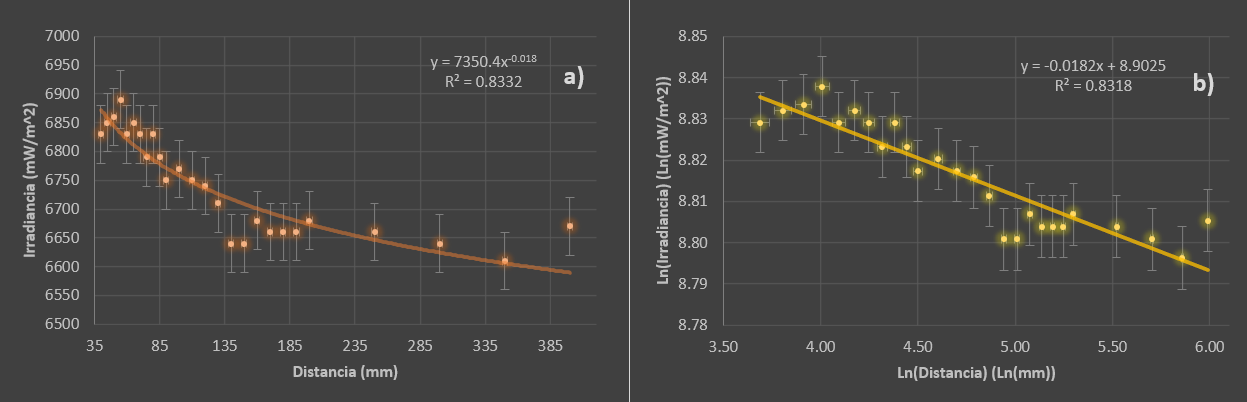
\includegraphics[width=1\linewidth]{Grafico PL colimado.png}
    \caption{a) Gráfico d vs R con incertidumbres \qquad b) Gráfico ln(d) vs ln(R) con incertidumbres}
    \label{fig:enter-label}
\end{figure}

Nótese que obtenemos una expresión de la irradiancia de la forma $I = 7350.4r^{-0.018} \approx \lim_{m\rightarrow0^+} \dfrac{\Gamma_0}{r^m}$. Por lo que podemos asumir que el laser es un haz colimado pues se ha cumplido que la irradiancia es prácticamente independiente de la distancia, al menos en nuestro intervalo de estudio, aunque para nosotros lo más acertado es considerar este exponente ($-0.0182\pm 0.002$) en el radio para poder considerar esta ligera divergencia que presenta nuestro laser; por otro lado en el gráfico linealizado obtuvimos la ecuación $\ln I = -0.0182\ln r + 8.9025$, nuevamente de aquí es más sencillo obtener la incertidumbre de m que acorde a los parámetros de la regresión lineal $\Delta m = 0.001673305 \approx 0.002
$. De modo que finalmente nuestra irradiancia del LED queda determinada por

\begin{mdframed}
    \begin{equation}
        I = \frac{7350.4}{r^{0.0182\pm0.002}}
    \end{equation}
\end{mdframed}

\subsection{Diferencia entre la fuente puntual y el haz colimado}

Finalmente, para comparar el comportamiento de ambas fuentes de forma más visual, se graficaron ambos conjuntos de datos sin linealizar, pero de forma normalizada, es decir, cada conjunto de datos se dividió por el dato de mayor valor para que el máximo tuviera un valor unitario. Debido al tamaño de la tabla podrá usted lector visualizarla en el anexo, a continuación se muestra el gráfico de ambos comportamientos. \\

\begin{figure}[H]
    \centering
    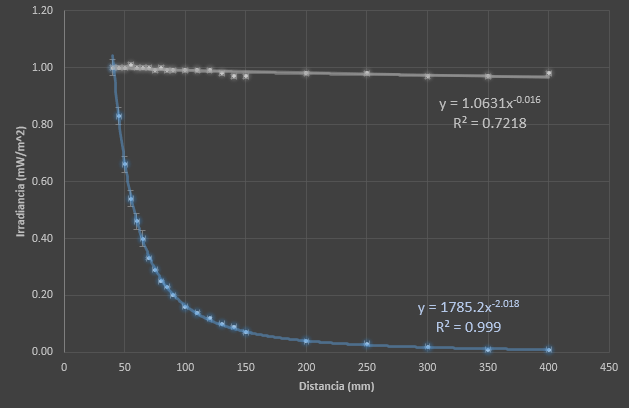
\includegraphics[width=1\linewidth]{Puntual vs Colimado.png}
    \caption{Gráfico normalizado $r$ vs $I$ de la fuente puntual (línea azul) en contraste del haz colimado (línea blanca)}
    \label{fig:enter-label}
\end{figure} \\

Se observa que la irradiancia del LED, al actuar como una fuente puntual, es significativamente alta a distancias cortas, pero disminuye abruptamente a medida que la distancia aumenta, en concordancia con la dependencia cuadrática esperada. En contraste, la irradiancia del haz colimado (láser) permanece prácticamente constante a lo largo de las distintas mediciones, lo que concuerda con el comportamiento teórico asociado a un exponente cercano a cero en la distancia.





\section{Conclusiones}
Los resultados experimentales obtenidos en este trabajo corroboran de manera contundente los modelos teóricos fundamentales que describen la propagación de la luz para fuentes puntuales y haces colimados. En el caso de la fuente puntual, representada por un LED, se verificó empíricamente la Ley Inversa al Cuadrado, lo que confirma su comportamiento como emisor isotrópico (frente de onda esférico) de radiación. La dependencia de la irradiancia con la distancia se ajustó a una relación potencial con un exponente de $-1.944 \pm 0.006$, un valor notablemente cercano al valor teórico de -2, lo que refuerza la validez del modelo y la precisión de las mediciones. En contraste, el haz colimado, generado por un láser, exhibió una irradiancia que se mantuvo prácticamente constante a lo largo de las distintas distancias de medición. Este comportamiento concuerda con la teoría de haces gaussianos y la mínima divergencia esperada en este tipo de fuentes. El ajuste de la irradiancia en función de la distancia reveló un exponente de $-0.0182 \pm 0.002$, lo que indica una muy ligera divergencia del haz real en comparación con lo que se le puede atribuir a una fuente de divergencia importante (como en este caso el led). Esta pequeña desviación del comportamiento ideal de un haz perfectamente colimado puede atribuirse a factores como las imperfecciones ópticas del sistema o los efectos de la difracción.

La comparación directa de la irradiancia normalizada para ambas fuentes ilustra de manera clara la diferencia fundamental en su comportamiento. Mientras que la fuente puntual muestra una rápida disminución de la irradiancia con la distancia, el haz colimado mantiene una irradiancia constante (al menos en nuestro intervalo de estudio que comprende desde los $(40\pm2)mm$ hasta los $(400\pm2)mm$), lo que destaca las ventajas de este último para aplicaciones que requieren la entrega de energía concentrada a distancias relativamente grandes. Los resultados obtenidos contribuyen al conocimiento fundamental de la óptica clásica y proporcionan herramientas valiosas para el desarrollo de nuevas tecnologías.

Como posible extensión de este trabajo, se podría considerar la investigación del comportamiento de las fuentes de luz a distancias mayores, así como el efecto de diferentes condiciones ambientales, como la temperatura o la humedad, en la propagación de la luz. Además, se podrían explorar otras características de las fuentes de luz, como la coherencia espacial y temporal, para obtener una caracterización más completa.


\begin{thebibliography}{20}

\bibitem[1]{}
E. Barrios, A. Hernández, R. Ramírez, *Propagación de la luz y Radiometría*, 2024.  \url{https://tsikbal.github.io/Paginas/Areas/Fisica/Optica/Optica_Geometrica/Radiometria.html}

\end{thebibliography}


\section*{Anexo}

\begin{mdframed}
 \begin{equation}
    \text{lin}(r) = \frac{\Delta r}{r}
\end{equation}
\end{mdframed}

Donde $r$ es la incertidumbre absoluta de la distancia, y $r$ la medición de la distancia.
\begin{mdframed}
\begin{equation}
    \text{lin}(I) = \frac{\Delta I}{I}
\end{equation}
\end{mdframed}

Donde $I$ es la incertidumbre absoluta de la Irradiancia, y $I$ la medición de la distancia.


Dado que lo que se requiere es la incertidumbre de $m$, primero de la ecuación (10) la despejamos, obteniendo:

\begin{mdframed}
\begin{equation}
    m = \frac{\ln(K) - \ln(I)}{\ln(r)}
\end{equation}
\end{mdframed}

Posteriormente, se propaga la incertidumbre respecto de las variables $I$ y $r$ (que son las mediciones del experimento) y tomando $K$ como constante. Así:

\begin{mdframed}
\begin{equation}
    \text{nom}(m) = \sqrt{\left(\frac{\Delta I}{I \ln(r)}\right)^2 + \left(\frac{\Delta r( \ln(K)-\ln(I))}{r (\ln(r))^2}\right)^2}
\end{equation}
\end{mdframed}

Dado que la fórmula de normalización para cada conjunto de datos es:

\begin{mdframed}
\begin{equation}
    I_{\text{norm}} = \frac{I - \text{Fondo}}{I_{\text{max}}}
\end{equation}
\end{mdframed}

Donde $I$ es la medición directa de Irradiancia, $\text{Fondo}$ es la irradiancia de fondo e $I_{\text{max}}$ es la irradiancia máxima registrada. La incertidumbre correspondiente, asumiendo que la irradiancia de Fondo no cuenta con incertidumbre, es:

\begin{mdframed}
\begin{equation}
    I_{\text{norm}} = \frac{\Delta I}{I_{\text{max}}}
\end{equation}
\end{mdframed}

Donde $I$ es la incertidumbre absoluta de la irradiancia medida.



\end{document}